\section*{Exercice 2 (5 points)}
	
\subsection*{1. Calculer la probabilité que le client ait souscrit à l’assurance complémentaire et ait acheté la coque.}
	
On peut dresser l’arbre pondéré de probabilités :
\begin{center}
	\begin{tikzpicture}
[level 1/.style={level distance=2cm,
		sibling distance=3cm},
	level 2/.style={level distance=2.5cm,
		sibling distance=1.5cm}]
	\node {} [grow'=right]
	child {node {$A$}
		child {node {$C$}
			edge from parent node[above] {$0,2$}
		}
		child {node {$\overline C$}
			edge from parent node[below] {$0,8$}
		}
		edge from parent node[above] {$0,4$}
	}
	child {node {$\overline A$}
		child {node {$C$}
			edge from parent node[above] {$\dfrac13$}
		}
		child {node {$\overline C$}
			edge from parent node[below] {$\dfrac23$}
		}
		edge from parent node[below] {$0,6$}
	}
	;
\end{tikzpicture}
\end{center}
	
La probabilité que le client ait souscrit à l’assurance complémentaire et ait acheté la coque est $p(A\cap C)=0,4 \times 0,2 = 0,08$.
	
\subsection*{2. Montrer que $P(C) = 0,28$.}
	
	D’après la loi des probabilités totales :
	\[
	P(C) = P(A \cap C) + P(\overline{A} \cap C) = P(A) \times P_A(C) + P(\overline{A}) \times P_{\overline{A}}(C) = 0,4 \times 0,2 + 0,6 \times \dfrac{1}{3} = 0,08 + 0,2 = 0,28
	\]
	
\subsection*{3. Le client interrogé a acheté la coque. Quelle est la probabilité qu’il n’ait pas souscrit à l’assurance complémentaire ?}
	
Il faut calculer $P_C(\overline{A}) = \dfrac{P(C \cap \overline{A})}{P(C)} = \dfrac{0,20}{0,28} = \dfrac{10}{14} = \dfrac{5}{7}$.
	
\subsection*{4. Déterminer la dépense moyenne d’un client de ce magasin ayant acheté un smartphone de la marque Pomme.}
	
On pourra noter $X$ la variable aléatoire qui représente la dépense en euros d’un client de ce magasin ayant acheté un smartphone de la marque Pomme.\\
$X$ peut prendre les valeurs : $870, 850, 820$ et $800$ avec les probabilités respectives $0,08; 0,32; 0,2 ; 0,4$.\\
La dépense moyenne par client ayant acheté un smartphone est donc :
	\[E(X)=
	870 \times 0,08 + 850 \times 0,32 + 820 \times 0,2 + 800 \times 0,4 = 69,6 + 272 + 164 + 320 = 825,60 \text{€}
	\]
	
